
%%%%%%%%%%%%%%%%%%%%%%% file typeinst.tex %%%%%%%%%%%%%%%%%%%%%%%%%
%
% This is the LaTeX source for the instructions to authors using
% the LaTeX document class 'llncs.cls' for contributions to
% the Lecture Notes in Computer Sciences series.
% http://www.springer.com/lncs       Springer Heidelberg 2006/05/04
%
% It may be used as a template for your own input - copy it
% to a new file with a new name and use it as the basis
% for your article.
%
% NB: the document class 'llncs' has its own and detailed documentation, see
% ftp://ftp.springer.de/data/pubftp/pub/tex/latex/llncs/latex2e/llncsdoc.pdf
%
%%%%%%%%%%%%%%%%%%%%%%%%%%%%%%%%%%%%%%%%%%%%%%%%%%%%%%%%%%%%%%%%%%%


\documentclass[runningheads,a4paper]{llncs}

\usepackage{amssymb}
\setcounter{tocdepth}{3}
\usepackage{graphicx}

\usepackage{url}
\urldef{\mailsa}\path|{dsand, karkare}cse.iitk.ac.in|
%\urldef{\mailsb}\path|anna.kramer, leonie.kunz, christine.reiss, nicole.sator,|
%\urldef{\mailsc}\path|erika.siebert-cole, peter.strasser, lncs}@springer.com|    
\newcommand{\keywords}[1]{\par\addvspace\baselineskip
\noindent\keywordname\enspace\ignorespaces#1}

%%%%%% Non recom packages
\usepackage{pstricks}
\usepackage{pst-node}
\usepackage{pst-rel-points}
\usepackage{latexsym}
\usepackage{verbatim}
\usepackage{amsmath}

%%%%%%%%%%%%%%%%%%%%%%%%%%%%%%%%%%%%%%%%
%%%%%%% theorams and definitions %%%%%%%
%%%%%%%%%%%%%%%%%%%%%%%%%%%%%%%%%%%%%%%%
\newtheorem{defn}{Definition}[section]
\newtheorem{exmpl}{Example}[section]
\newtheorem{prop}{Property}[section]
%%%%%%%%%%%%%%%%%%%%%%%%%%%%%%%%%%%%%%%%
%%%%%%% New Commands %%%%%%%%%%%%%%%%%%
%%%%%%%%%%%%%%%%%%%%%%%%%%%%%%%%%%%%%%%%
\newcommand{\cmt}[1]{} % commented out stuff
% Review these names
\newcommand{\p}{\mbox{\tt p}}
\newcommand{\nO}{\mbox{\tt n1}}
\newcommand{\nT}{\mbox{\tt n2}}
\newcommand{\myt}{\mbox{\tt t}}
\newcommand{\q}{\mbox{\tt q}}
\newcommand{\s}{\mbox{\tt s}}
\newcommand{\myr}{\mbox{\tt r}}

\newcommand{\B}{\mbox{\tt B}}
\renewcommand{\a}{\mbox{\tt a}}
\renewcommand{\b}{\mbox{\tt b}}
\renewcommand{\c}{\mbox{\tt c}}
\renewcommand{\d}{\mbox{\tt d}}
\newcommand{\m}{\mbox{\tt m}}

\newcommand{\drct}{\ensuremath{D}}
\newcommand{\indrct}{\ensuremath{I}}
\newcommand{\heap}{\ensuremath{\mathcal{H}}}
\newcommand{\fields}{\ensuremath{\mathcal{F}}}
\newcommand{\upath}{\ensuremath{\mathcal{U}}}
\newcommand{\shape}{\mbox{shape}}
\newcommand{\nat}{\ensuremath{\bbbn}}

\newcommand{\mwedge}{\; \wedge \;}
\newcommand{\mvee}{\; \vee \;}
\newcommand{\mcup}{\; \cup \;}
\newcommand{\mjoin}{\; \Join \;}
\newcommand{\mbackslash}{\; \backslash \;}
\newcommand{\subC}{\mbox{\scalebox{.6}{\Cycle}}}
\newcommand{\subD}{\mbox{\scalebox{.6}{\Dag}}}

\newcommand{\epsilonset}{\ensuremath{\{\epsilon\}}}
\newcommand{\epsilonpairset}{\ensuremath{\{\epsilon,\epsilon\}}}

\newcommand{\dout}{\mbox{\footnotesize\em out}}
\newcommand{\din}{\mbox{\footnotesize\em in}}
\newcommand{\dkill}{\mbox{\footnotesize\em kill}}
\newcommand{\dgen}{\mbox{\footnotesize\em gen}}

\newcommand{\GenC}[1]{\ensuremath{{#1}_{\subC}^{\dgen}}}
\newcommand{\GenD}[1]{\ensuremath{{#1}_{\subD}^{\dgen}}}
\newcommand{\KillC}[1]{\ensuremath{{#1}_{\subC}^{\dkill}}}
\newcommand{\KillD}[1]{\ensuremath{{#1}_{\subD}^{\dkill}}}
\newcommand{\InC}[1]{\ensuremath{{#1}_{\subC}^{\din}}}
\newcommand{\InD}[1]{\ensuremath{{#1}_{\subD}^{\din}}}
\newcommand{\OutC}[1]{\ensuremath{{#1}_{\subC}^{\dout}}}
\newcommand{\OutD}[1]{\ensuremath{{#1}_{\subD}^{\dout}}}

\newcommand{\project}[2]{\red
  \ensuremath{#1\triangleright\!\!#2}}
\newcommand{\num}[1]{\red
  \ensuremath{|#1|}}
\newcommand{\first}[1]{\ensuremath{#1. \mathrm{fst}}}
\newcommand{\second}[1]{\ensuremath{#1. \mathrm{snd}}}

\newcommand{\remOne}[2]{\red \ensuremath{#1 \ominus #2}}
\newcommand{\remAll}[2]{\red \ensuremath{#1\ominus #2}}

\newcommand{\mb}[1]{\mbox{{\tt #1}}}
\newcommand{\D}[2]{\mb{$D$}[\mb{#1},\mb{#2}]}
\newcommand{\I}[2]{\mb{$I$}[\mb{#1},\mb{#2}]}
\newcommand{\DFM}[2]{\mb{$D_F$}[\mb{#1},\mb{#2}]}
\newcommand{\IFM}[2]{\mb{$I_F$}[\mb{#1},\mb{#2}]}
\newcommand{\DFMI}[2]{\mb{$D_{F}$}^{\tt in}[\mb{#1},\mb{#2}]}
\newcommand{\IFMI}[2]{\mb{$I_{F}$}^{\tt in}[\mb{#1},\mb{#2}]}
\newcommand{\DFMO}[2]{\mb{$D_{F}$}^{\tt out}[\mb{#1},\mb{#2}]}
\newcommand{\IFMO}[2]{\mb{$I_{F}$}^{\tt out}[\mb{#1},\mb{#2}]}
\newcommand{\Tree}{{\tt Tree}}
\newcommand{\Dag}{{\tt Dag}}
\newcommand{\Cycle}{{\tt Cycle}}
\newcommand{\upstmt}[1]{{\tt p$\rightarrow$f = #1}}
\newcommand{\TV}{{\tt TrueVars}}
\newcommand{\fieldD}[2]{\ensuremath{{#1}_{#2}^\drct}}
\newcommand{\fieldI}[3]{\ensuremath{{#1}_{#2}^{\indrct#3}}}
\newcommand{\range}[3]{\ensuremath{{#1} \leq {#2} \leq {#3}}}
\newcommand{\U}{{\rm Unknown}}
\newcommand{\fig}[1]{\includegraphics[scale=.5]{#1}}
\newcommand{\false}{\textbf{False}}
\newcommand{\true}{\textbf{True}}

\newcommand{\sub}[2]{\ensuremath{{#1}_{#2}}}

\begin{document}

\mainmatter  % start of an individual contribution

% first the title is needed
\title{Precise Shape Analysis using Field Sensitivity}

% a short form should be given in case it is too long for the running head
\titlerunning{Precise Shape Analysis using Field Sensitivity}

% the name(s) of the author(s) follow(s) next
%
% NB: Chinese authors should write their first names(s) in front of
% their surnames. This ensures that the names appear correctly in
% the running heads and the author index.
%
\author{Sandeep Dasgupta \and Amey Karkare}
%
\authorrunning{Precise Shape Analysis using Field Sensitivity}
% (feature abused for this document to repeat the title also on left hand pages)

% the affiliations are given next; don't give your e-mail address
% unless you accept that it will be published
\institute{Department of Computer Science and Engineering,\\
Indian Institute of Technology Kanpur, Kanpur, India\\
\mailsa\\
%\mailsb\\
%\mailsc\\
\url{http://www.cse.iitk.ac.in}}


\toctitle{Lecture Notes in Computer Science}
\tocauthor{Authors' Instructions}
\maketitle

%%%%%%%%%%%%%%%%%%%%%%%%%%%%%%%%%%%%%%%%%%%%%%%%%%%%%
\section{Termination Criteria}
%%%%%%%%%%%%%%%%%%%%%%%%%%%%%%%%%%%%%%%%%%%%%%%%%%%%%

\newcommand{\GenSym}{\Psi}
\newcommand{\KillSym}{\gamma}

The termination of computation of boolean functions for Cycle and Dag can be proved using the associativity 
and distributivity of the bollean operators ($\vee$ and $\wedge$).
Consider Fig.~\ref{fig:flowdiag}(a) which shows a basic block b with its in and out sets, IN(b) and OUT(b) respectively.
The boolean formulas $\GenSym$ and $\KillSym$ respectively denote the gen and kill sets corresponding to basic bloack b. Let f denotes the 
boolean formula at a program poin before executing b. Figure~\ref{fig:flowdiag}(b) shows the in and out sets generated in each iteration 
of the data flow analysis. As depicted in Fig.~\ref{fig:flowdiag}(b), the boolean functions reeached fixed-point after the second iteration.  
\begin{figure}
\centering
\begin{tabular}{@{}lc@{}}
\scalebox{.5} {
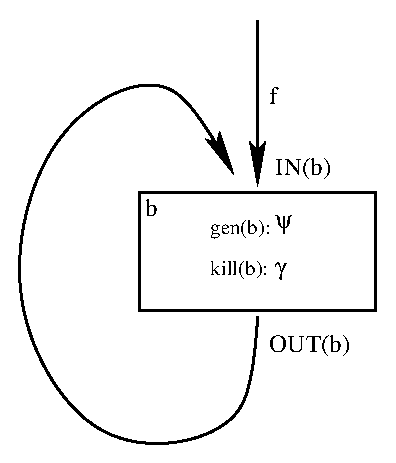
\includegraphics[scale=1]{Figure/figure_1} }
&
\scalebox{.75} {
\begin{tabular}{|c|c|c|}
\hline
Iteration & IN(b) & OUT(b) \\ \hline
\hline
$1$ & $f$									& $(f \wedge \KillSym) \vee \GenSym$ \\ \hline 
$2$ & $f \vee ((f \wedge \KillSym) \vee \GenSym)$	& 
			$\begin{array}{cl}
				& ((f \vee ((f \wedge \KillSym) \vee \GenSym)) \wedge \Kill) \vee \GenSym \\
			 	=& (((f \vee (f \wedge \KillSym)) \vee \GenSym) \wedge \Kill) \vee \GenSym \\
			 	=& ((f \vee \GenSym) \wedge \KillSym) \vee \GenSym \\
			 	=& (f \vee \GenSym \vee \Gen) \wedge (\KillSym \vee \GenSym) \\
			 	=& (f \vee \GenSym) \wedge (\KillSym \vee \GenSym) \\
			 	=& (f \wedge \KillSym) \vee \GenSym \\
			\end{array}$ \\ \hline 
$3$ & $f \vee ((f \wedge \KillSym) \vee \GenSym)$	& $(f \wedge \KillSym) \vee \GenSym$ \\ \hline
\end{tabular}} \\ \\
 \footnotesize (a) Data Flow & \footnotesize (b) Data flow values per iteration \\
\end{tabular}
\label{fig:flowdiag}
\caption{The termination of computation of boolean functions}
\end{figure}



\end{document}
